\section{Verification and validation}
\label{ss:c3}

\subsection{Flow and Heat Transfer verification and validation}

\subsubsection{Nek5000 - Canonical cases}
To verify the fluid flow model and the solution transfer, we have devised two cases, including a single pebble and a two pebble case. The Nek5000-MOOSE coupling was verified to yield the same results as stand-alone Nek5000 conjugate heat transfer results. We note that work in Cardinal was based on previous work conducted on Nek5000-MOOSE coupling \cite{novak2018preliminary}. Single pebble (Figure~\ref{f:vvf1}) and two pebble (Figure~\ref{f:vvf2}) cases were used to verify the solution transfer. They were also used to verify the coupling with OpenMC and BISON coupling. For instance, the neutronics results showed a clear bias between pebbles and a tilt induced by the temperature gradient.

\begin{figure}[!h]
\centering
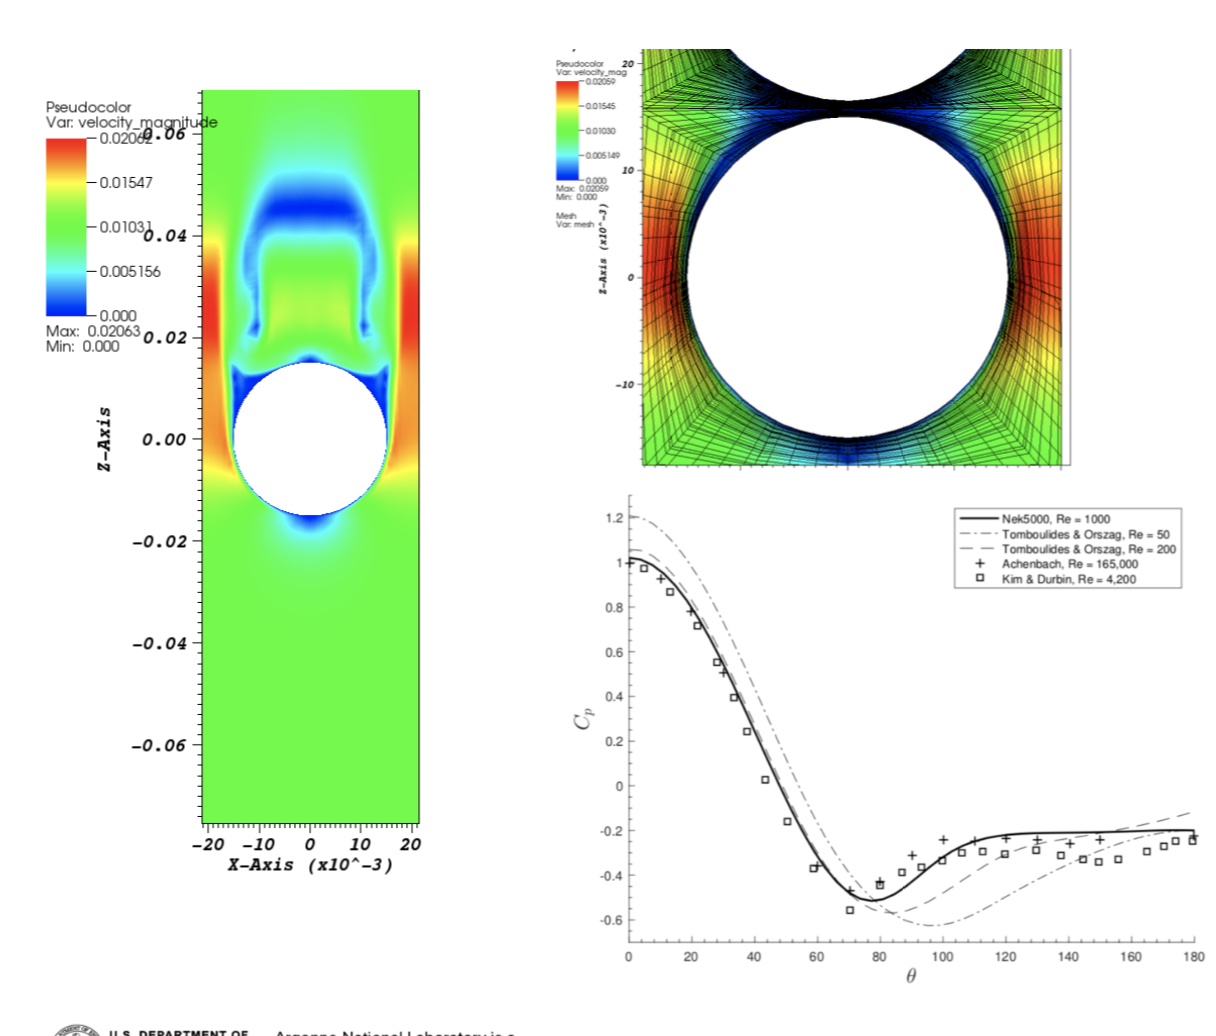
\includegraphics[clip=true,width=0.9\textwidth]{Figures/pb_vv1}
\caption{Verification test - Single pebble and comparison with experiment.}
\label{f:vvf1}
\end{figure}

\begin{figure}[!h]
\centering
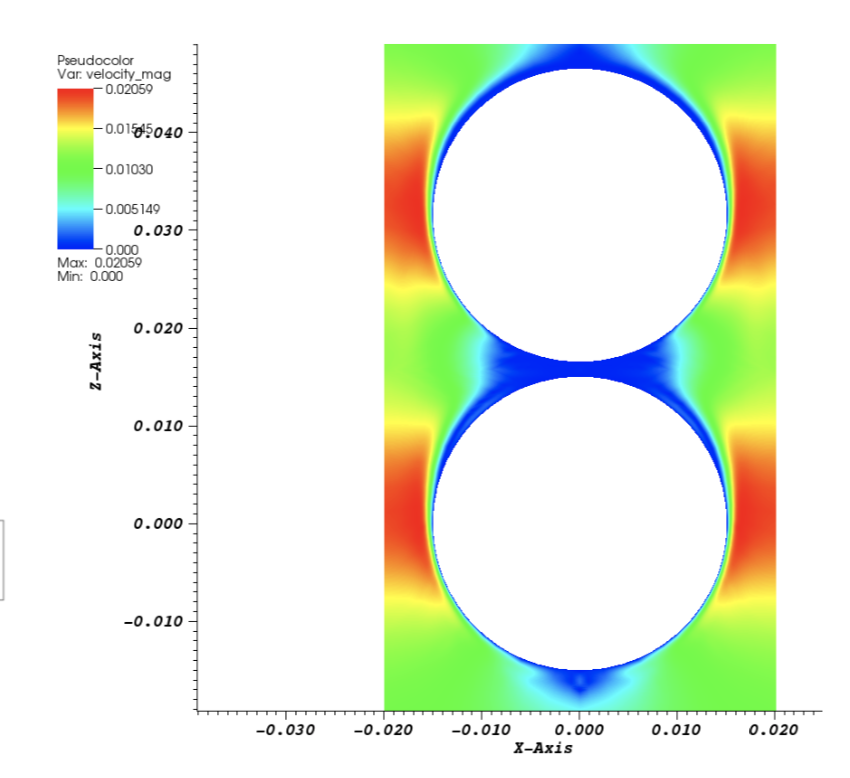
\includegraphics[clip=true,width=0.6\textwidth]{Figures/pb_vv2}
\caption{Verification test - Two pebbles.}
\label{f:vvf2}
\end{figure}

Selected results from the single pebble case were also compared with results from experimental and computational studies carried out using a similar geometry (Figure~\ref{f:vvf1}). A well-quantified quantity for flow over a single-sphere is the averaged stream-wise velocity along the domain axial centerline. Figure~\ref{f:vvf1} compares our result with completed numerical results. The figure shows the profile generated from DNS data in \cite{fick2017investigation} at $Re = 3,700$ and shows the downstream location ($z=D$) and magnitude of the maximum recirculation (i.e. negative streamwise) velocity for LES and DES data generated at $Re = 10,000$. One can see that for increasing Reynolds number, the magnitude of the recirculation velocity increases, while the downstream distance from the sphere where this maximum occurs, decreases. We do not quantify this trend's specific dependence on the Reynolds number here, but our result is consistent with the literature.

\subsubsection{NekRS-BISON coupling}

We have also compared directly results obtained with the NekRS version of Cardinal versus Nek5000. The case setup is identical to the one used for the verification of the MOOSE-Nek5000 coupling. Some results for the temperature distribution are shown in Figure~\ref{f:nrs1}.

\begin{figure}[!h]
\centering
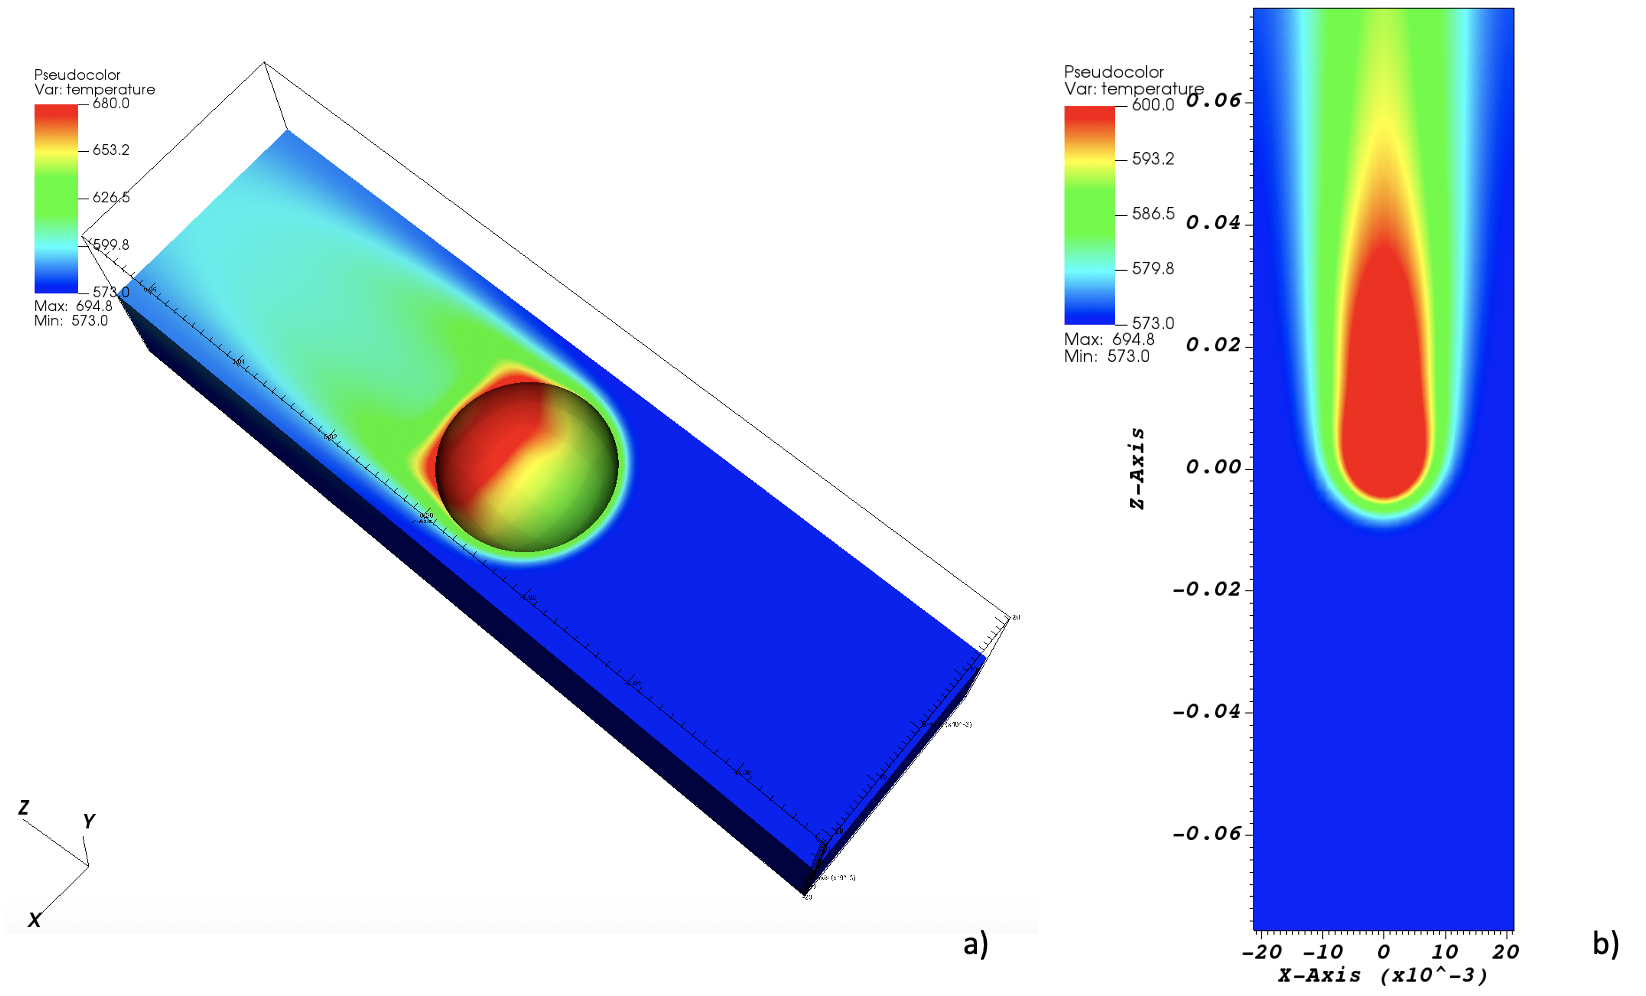
\includegraphics[clip=true,width=0.9\textwidth]{Figures/nrs_vv1}
\caption{Verification test - Single pebble result. a) 3D temperature distribution in the whole domain. b) Cross section at $y=0.016 m$.}
\label{f:nrs1}
\end{figure}

Figure~\ref{f:nrs2} presents single pebble results in Cardinal,  where the fluid is simulated in NekRS, and the interior of the pebble is simulated with BISON (in this case with the heat conduction module of MOOSE). Results are compared with solutions obtained with Nek5000 stand-alone, using the conjugate heat transfer feature of the code. Temperature profiles are compared on a line at $y=0.016 m$ and $x=0 m$ (we note that the domain is centered at the pebble center and the pebble diameter is $D=0.03 m$). We note that the results are nearly identical if a quadratic representation of the surface is employed.

\begin{figure}[!h]
\centering
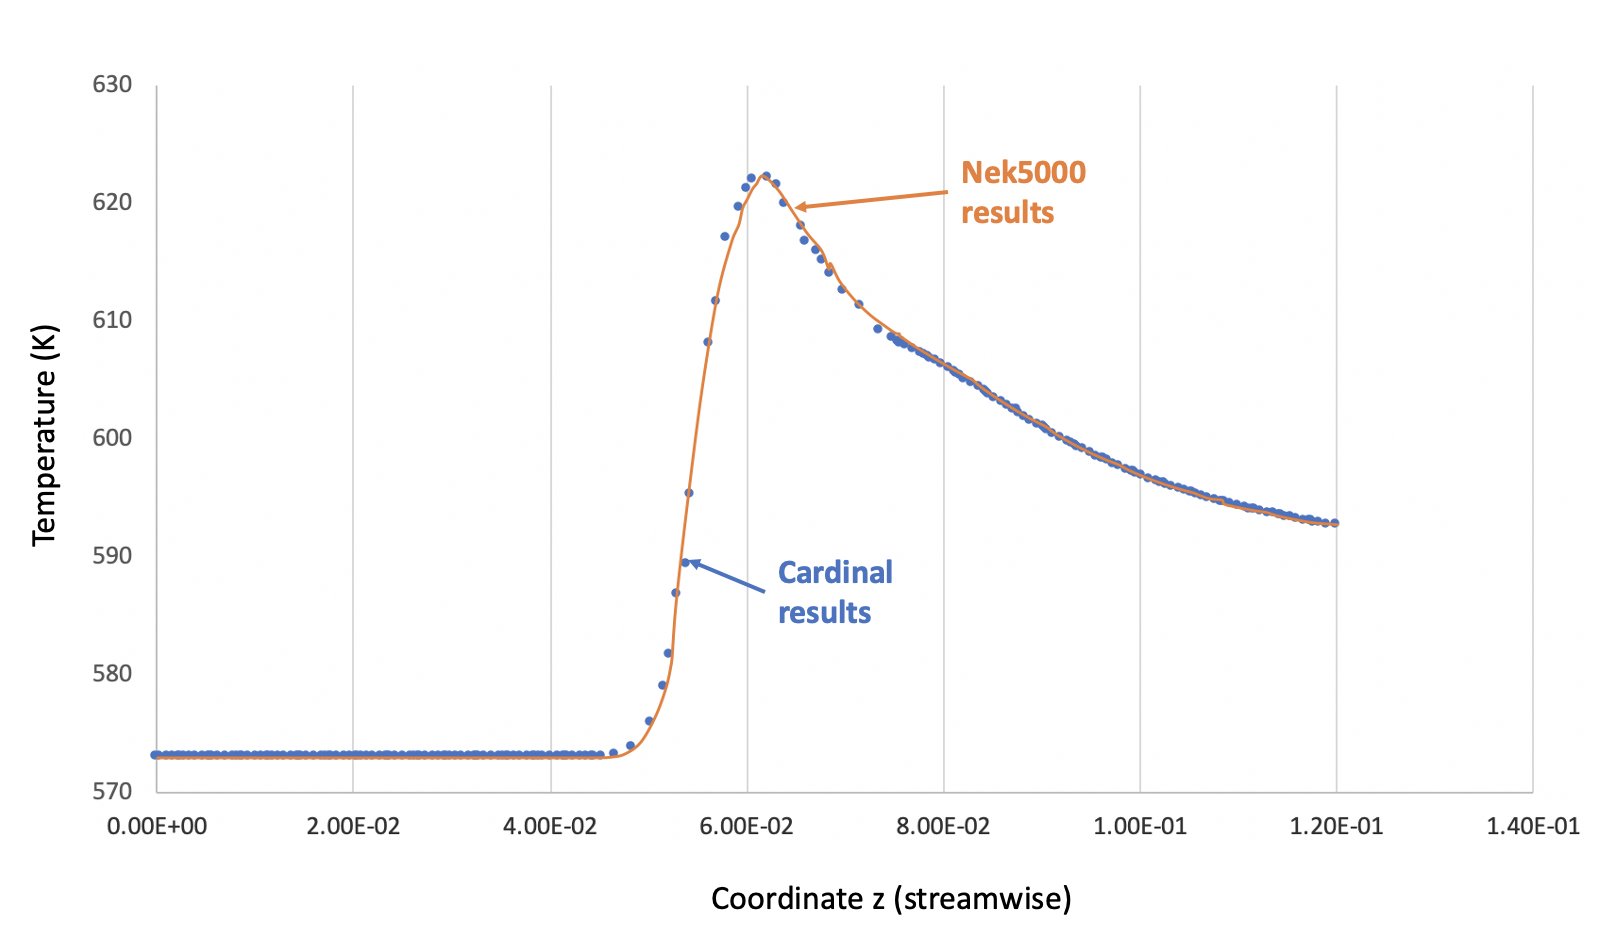
\includegraphics[clip=true,width=0.9\textwidth]{Figures/nrs_vv2}
\caption{Verification test - Single pebble comparison with standalone Nek5000 results. }
\label{f:nrs2}
\end{figure}

\subsubsection{Pebble beds}

Over the past several years, NEAMS has dedicated several efforts to the modeling and simulation of the detailed flow in a pebble bed. For instance, Fick et al. \cite{fick2017direct}  performed a complete Direct Numerical Simulation of pebble bed flow. Complete statistical data was obtained from this DNS study, with an investigation of low-frequency temporal instabilities. However, Fick's study \cite{fick2017direct} used a structured pebble bed, which limits its application. Nonetheless, it was compared against other available DNS data and proved Nek5000 can deliver high-quality simulation data for pebble beds. A more recent study was aimed at simulating the flow in a random pebble bed \cite{yildiz2020direct}. This random pebble bed geometry was obtained from an experiment conducted by Nguyen et al. \cite{nguyen2018time}. However, only a small section of the whole domain from the experiment was studied.

To create a pure hexahedral mesh for a random pebble bed is very challenging using the traditional blocking method. However, with the tet-to-hex meshing method, we can create a pure hexahedral mesh for this geometry. To reduce the total element count, chamfers are created at pebble-pebble interfaces. As discussed, the computational domain is only a small section of the whole experimental domain; therefore, we applied periodic boundary conditions at the inlet/outlet to mimic the upstream/downstream. Figure~\ref{f:tamu3} shows the instantaneous velocity field at cross-sections of the random pebble bed and the near-wall mesh at the pebble surface. In Figure~\ref{f:tamu4}, the flow field is very complex due to the randomly distributed pebbles. Despite the complexity of the geometry, the computational results compared favorably.

\begin{figure}[!h]
\centering
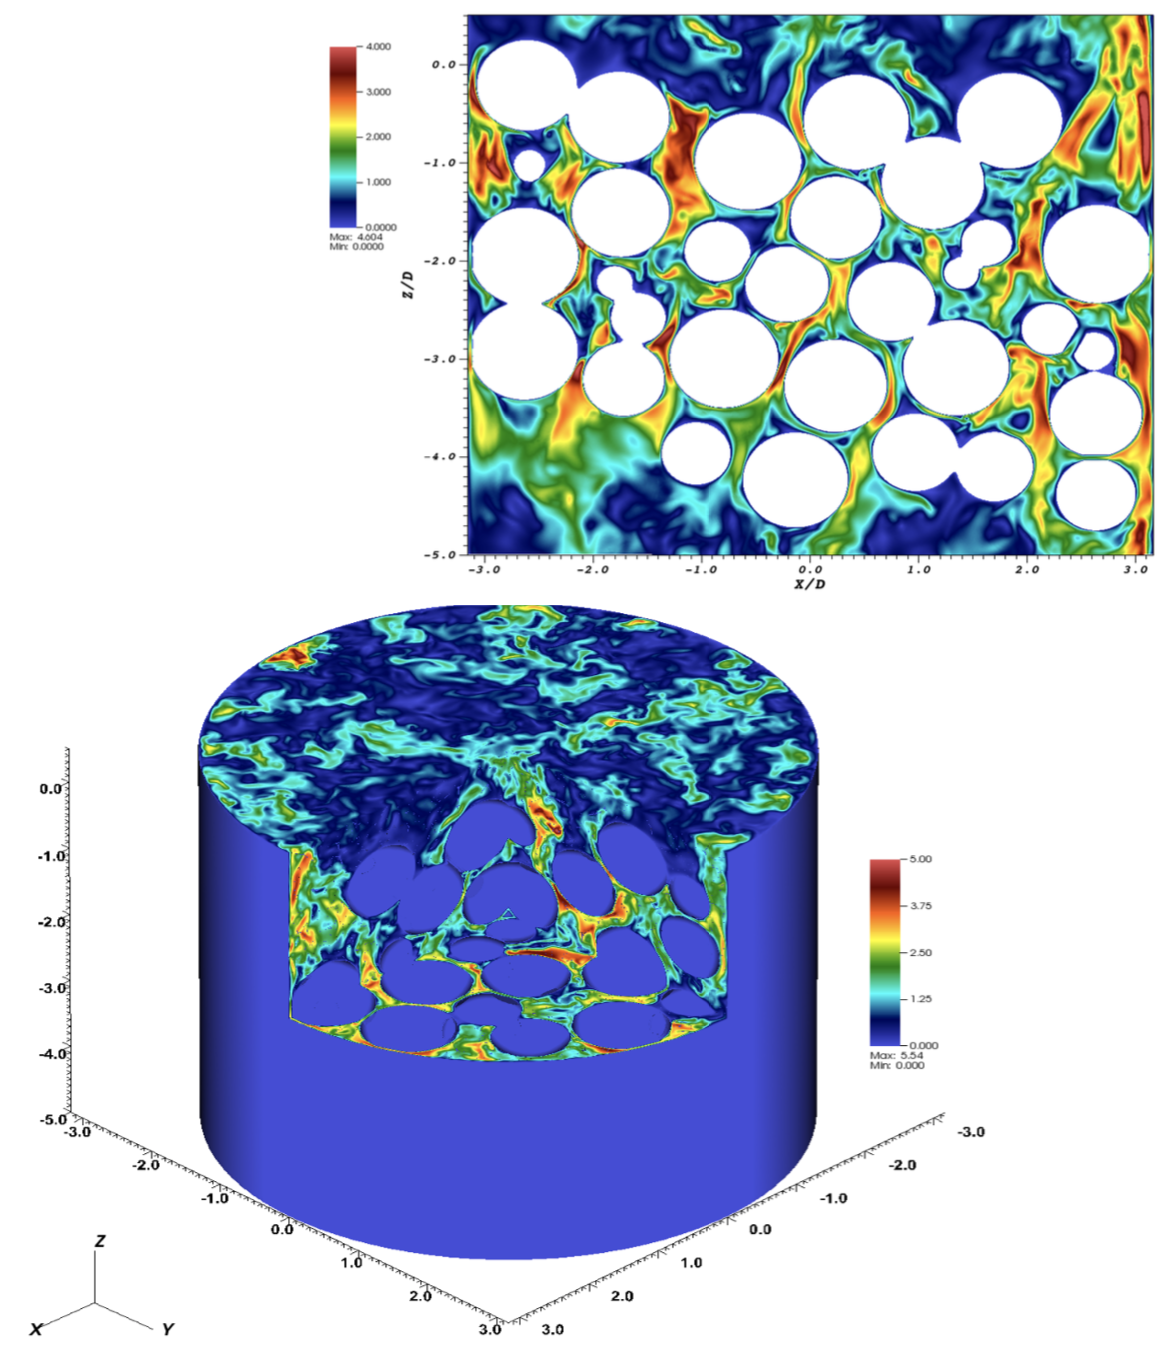
\includegraphics[clip=true,width=0.9\textwidth]{Figures/pb_tamu3}
\caption{TAMU experiment - Simulation results.}
\label{f:tamu3}
\end{figure}

\begin{figure}[!h]
\centering
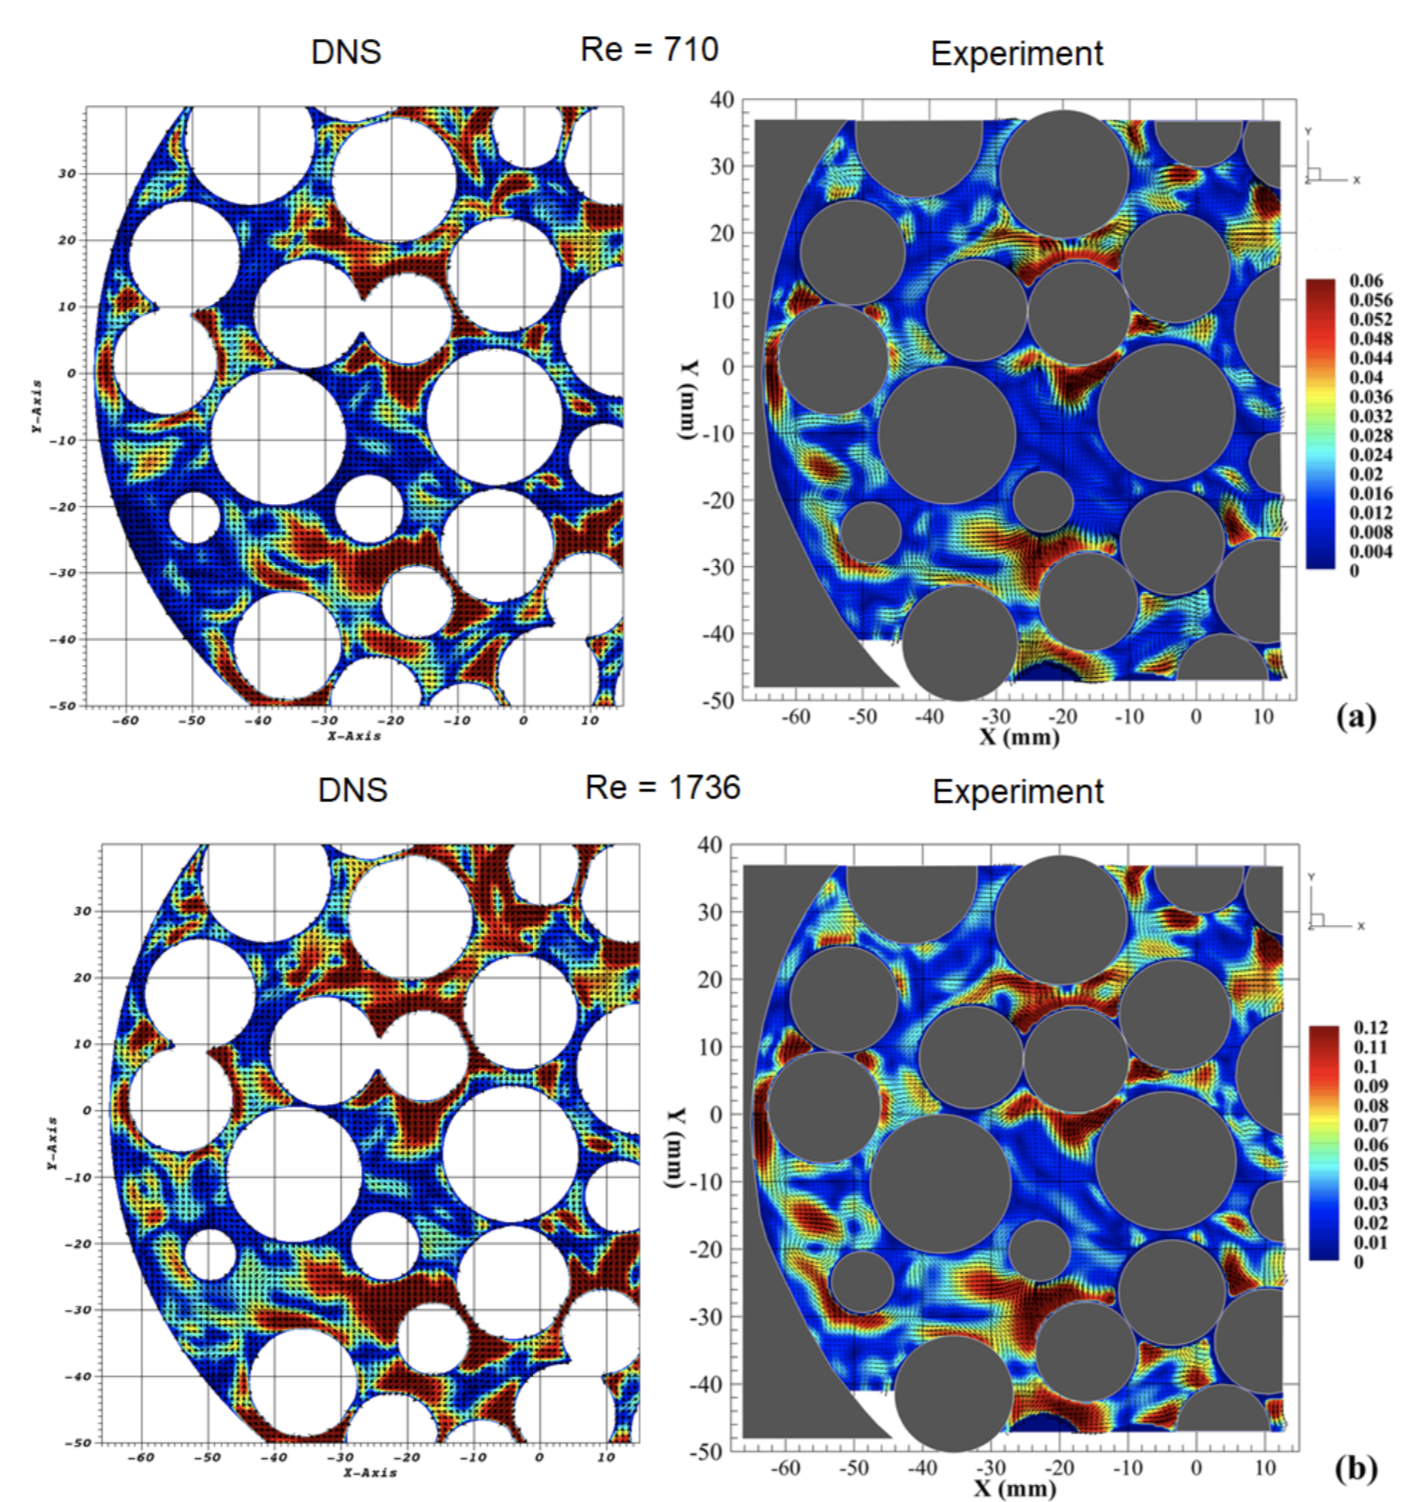
\includegraphics[clip=true,width=0.9\textwidth]{Figures/pb_tamu4}
\caption{TAMU experiment - Comparison with experiment. }
\label{f:tamu4}
\end{figure}

\subsection{Neutronics verification and validation}

We consider a pebble bed configuration similar to the pebble experiment in Figure~\ref{f:tamu3}.
We compare results from OpenMC versus results obtained with MCNP.

For this demonstration, the sizes and composition of the TRISO particles were based on TRISO
manufactured by Phillips et al. at INL \cite{phillips2010}.  Though these particles were developed
for the Advanced Gas Reactor (AGR) fuel, particles with the same specifications are used for FHR
test reactors and computations benchmarks \cite{charalampos2014}.  The pebbles' sizes and compositions were taken from the Mark-1 FHR reactor constructed at UC Berkeley
\cite{charalampos2014}.  Tables \ref{tab:triso_comp}, \ref{tab:pebble_comp},
\ref{tab:coolant_comp}, and \ref{tab:pebble_dims} show these specifications.

\begin{table}
  \centering
  \begin{tabular}{|ll|}
    \hline \hline
    \textbf{Fuel Region}	 & Total mass density = 10.5 g/cm3 \\
    \hline
    Isotope	     & Relative atom density \\
    U234	       & 0.0143 \\
    U235	       & 7.10 \\
    U238	       & 28.3 \\
    C	           & 14.1 \\
    O	           & 50.5 \\
    \hline \hline
    \textbf{Buffer Layer} & Total mass density = 1.0 g/cm3 \\
    \hline
    C	           & 100 \\
    \hline \hline
    \textbf{PyC Inner Layer}	   & Total mass density = 1.87 g/cm3 \\
    \hline
    C	           & 100 \\
    \hline \hline
    \textbf{SiC Layer}	   & Total mass density = 3.2 g/cm3 \\
    \hline
    C	           & 50.0 \\
    Si	         & 50.0 \\
    \hline \hline
    \textbf{PyC Outer Layer}	     & Total mass density = 1.6 g/cm3 \\
    \hline
    C	           & 100 \\
    \hline \hline
  \end{tabular}
  \caption{TRISO Composition}
  \label{tab:triso_comp}
\end{table}


\begin{table}
  \centering
  \begin{tabular}{|ll|}
    \hline \hline
    \textbf{Inner Graphite Core}	& Total mass density = 1.59 g/cm3 \\
    \hline
    Isotope	& Relative atom density \\
    C	& 100 \\
    \hline \hline
    \textbf{Outer Graphite Shell}	& Total mass density = 1.74 g/cm3 \\
    \hline
    C	& 100 \\
    \hline \hline
  \end{tabular}
  \caption{Pebble Composition}
  \label{tab:pebble_comp}
\end{table}


\begin{table}
  \centering
  \begin{tabular}{|ll|}
    \hline \hline
    \textbf{FLiBe}	      & Total mass density = 1.97 g/cm3 \\
    \hline
    Isotope	              & Relative atom density \\
    Li7	                  & 28.6 \\
    Li6	                  & 0.00286 \\
    Be9	                  & 14.3 \\
    F19	                  & 57.1 \\
    \hline \hline
  \end{tabular}
  \caption{Coolant Composition}
  \label{tab:coolant_comp}
\end{table}

\begin{table}
  \centering
  \begin{tabular}{|ll|}
    \hline \hline
    TRISO Particle Dimensions & \\
    \hline
    \textbf{Particle Diameter}	 & 400 $\mu$m \\
    \textbf{Buffer Layer Thickness} & 100 $\mu$m \\
    \textbf{PyC Inner Layer Thickness}	   & 35 $\mu$m \\
    \textbf{SiC Layer Thickness}	   & 35 $\mu$m \\
    \textbf{PyC Outer Layer Thickness}	     & 35 $\mu$m \\
    \hline \hline
    Pebble Dimensions & \\
    \hline
    \textbf{Pebble Diameter} & 30.0 mm \\
    \textbf{Inner Core Diameter} & 25.0 mm \\
    \textbf{Outer Shell Thickness} & 1.0 mm \\
    \hline \hline
  \end{tabular}
  \caption{TRISO And Pebble Dimensions}
  \label{tab:pebble_dims}
\end{table}

The resultant OpenMC model is shown in Figure~\ref{f:openmc_pebble}; the figure shows a close-up of a 2D slice of one pebble.  In this demo, the TRISO particles are packed in a regular, square lattice with the same overall packing fraction described by \cite{phillips2010}, rather than a randomized and/or irregular distribution.  This choice was made for computational efficiency since OpenMC can apply optimizations for particle (i.e., neutron) tracking in a regular lattice.  Some optimization methods have been developed specifically for building models with TRISO particles \cite{openmcdocs_triso}, and these will be used for future demonstrations.

\begin{figure}[!h]
\centering
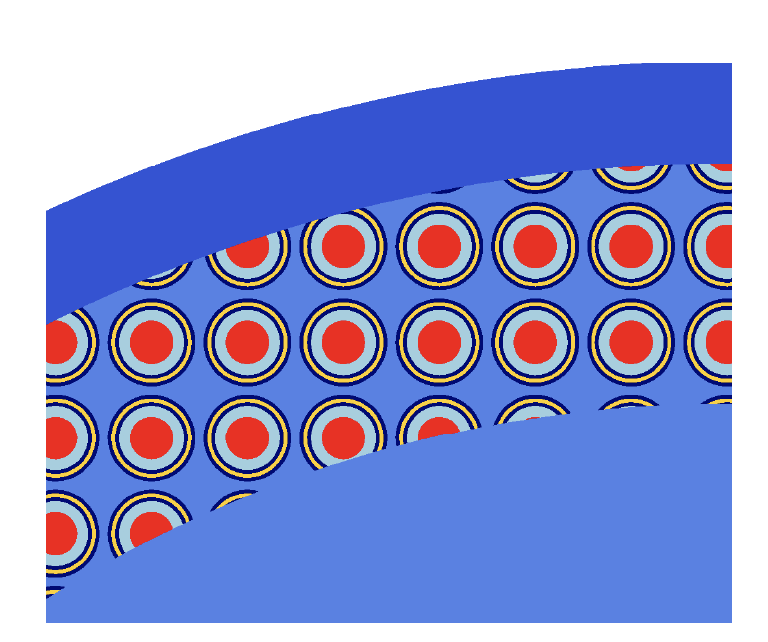
\includegraphics[clip=true,width=0.5\textwidth]{Figures/pebble_yz_cropped.png}
\caption{A 2D slice of the OpenMC model of an FHR pebble.  Red represents fuel, yellow represents
SiC, and blue represents graphite (where darker shades are more dense).}
\label{f:openmc_pebble}
\end{figure}

Table~\ref{tab:eigen} presents a comparisons for the $k$-eigenvalue computed with OpenMC and MCNP for various boundary condition combinations. We note the strong sensitivity to the radial boundary condition, given the small size of the domain. Overall results are consistent between the two codes.

\begin{table}
  \centering
  \begin{tabular}{|lcc|}
    \hline \hline
    MCNP &  & \\
    \hline
    Boundary conditions & Eigenvalue & \\
    \hline
    \textbf{r vacuum and z vacuum}         & 0.00357 & 0.000005 \\
    \textbf{r vacuum and z white}	         & 0.00463 & 0.000005 \\
    \textbf{r vacuum  and z reflective}    & 0.00448 & 0.000005 \\
    \textbf{r reflective and z reflective} & 1.10405 & 0.00005  \\
    \hline \hline
    OpenMC & & \\
    \hline
    Boundary conditions & Eigenvalue & \\
    \hline
    \textbf{r vacuum and z vacuum}         & 0.00356 & 0.00001 \\
    \textbf{r vacuum  and z reflective}    & 0.00451 & 0.00001 \\
    \textbf{r reflective and z reflective} & 1.10749 & 0.00082 \\
    \hline \hline
  \end{tabular}
  \caption{Eigenvalue for OpenMC and MCNP calculations}
  \label{tab:eigen}
\end{table}
